%!TEX root =  ../main.tex
\renewcommand{\columnseprule}{1.5pt}
\begin{multicols*}{2}
\rule[0.5\baselineskip]{0.4\textwidth}{1pt}
\noindent
\LabSection{Inverse of e}\label{sec:0803p}
\begin{exercises}{sec:0803p}
\lab{} Plot the graph of $y = e^x = y^\prime$.

\noindent
\begin{centering}
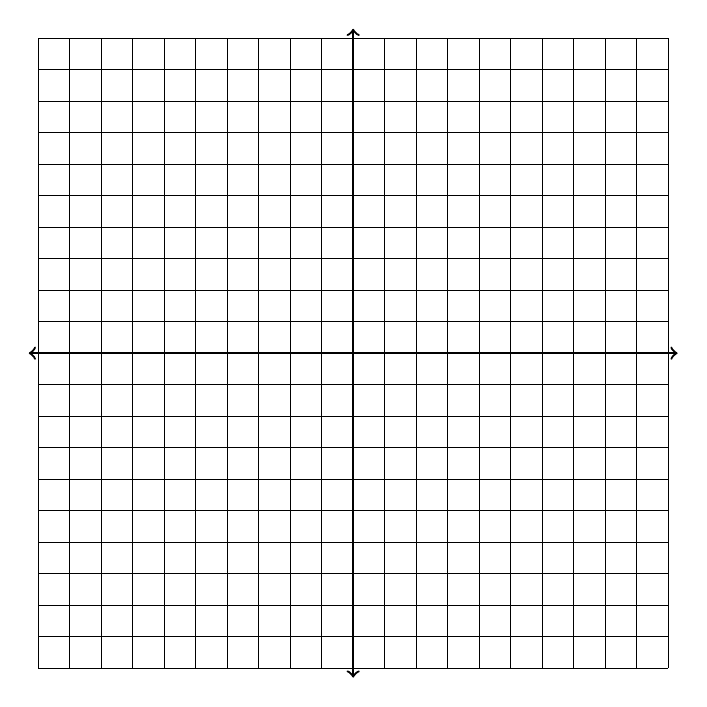
\begin{tikzpicture}[xscale=0.4,yscale=0.4]
	\draw [thick, <->] (-10.3,0) -- (10.3,0);
	\draw [thick, <->] (0,-10.3) -- (0,10.3);
	\draw [thin] (-10,-10) grid (10,10);
\end{tikzpicture}
\end{centering}


\lab{} Record the value of $1/e$ and check your graphs accuracy.

\vspace{2cm}
\lab{} We know that $\ln{x}$ [a.k.a. $\log_e{x}$] is the inverse function.  How can we graph an inverse from an original, numerically?


\vspace{2cm}
\lab{} State the property relating the derivative of an inverse to the derivative of the original.

\vspace{2cm}
\lab{} $e^x$ is special, because the height of the function is its derivative at every point.  Use the above properties to find the derivative of $\ln{x}$ verbally.

\vspace{2cm}
\lab{} Suppose $y$ is equal to a product of functions, $f\cdot{}g$.  How can we find $y\prime$?  Take the $\ln{}$ of both sides, and then the derivative, together called the \textbf{logarithmic derivative}.

\vspace{4cm}
\lab{} How can we find the derivative of $y = x^x$?  The exponent is not a constant, so we may not use the Power Rule.  The base is not a constant, so we may not use the derivative of $e^x$.  Find a way to find the derivative and use it to find the absolute minimum of the function.

\vspace{4cm}
\lab{} Describe in technical vocabulary what you think the point of this problem set is.

\end{exercises}
\end{multicols*}